%______________________________________________________________________________
%************************* HEADER *********************************************
\documentclass[]{scrreprt}
		
    
\usepackage{a4}
\usepackage[T1]{fontenc}
\usepackage[utf8]{inputenc}
\usepackage{lmodern}

\usepackage{subfigure}
\usepackage{epsfig}
\usepackage{graphicx}
\usepackage{graphics}
% \usepackage{array}
% \usepackage{units}
%\usepackage{cite}	 % Für Bibtex
\usepackage[noadjust]{cite}	 % Für Bibtex, noadjust: Keine Leerzeichen vor Referenz _[X]
\usepackage[]{placeins}  % für \FloatBarrier
\usepackage{amssymb} 
\usepackage[]{amsmath}   % Formelumgebung für begin{align]
% \usepackage{longtable}   % Mehrseitige Tabellen (Symbole)
\usepackage{booktabs}    % horizontale Linien in Tabellen
\usepackage{wrapfig}
% \usepackage{listings}    % Für Quellcode einbinden
\usepackage[onehalfspacing]{setspace}   % Einfacher Zeilenabstand für Tabellen

% \usepackage{tocbasic}
\usepackage[pdfpagelabels, plainpages=false]{hyperref} 
% \usepackage[linktocpage,pdfborderstyle={/S/U/W 1}]{hyperref}  % Links nur unterstrichen, nicht umrandet




% ---------------- header ----------------------
\usepackage{scrlayer-scrpage}
\automark{chapter}
\automark*{section}
\clearpairofpagestyles
\ihead{\headmark}
\ohead{\pagemark}

% ---------------- Sonstige Formatierung ----------------------
% \setlength{\parindent}{6pt} \linespread{1.3}  % Einrücken nach Absatz,  Zeilenabstand


% ---------------- Seiten-Einstellungen ----------------------
\usepackage{geometry}
\geometry{a4paper, top=25mm, left=35mm, right=25mm, bottom=25mm,
headsep=10mm, footskip=12mm}

\usepackage{blindtext}

\title{SWAT-EM}
\subtitle{Specific Winding Analyse Tool for Electrical Machines}
\author{Martin Baun}
\date{\today}

%************************* Titelseite *****************************************
\begin{document}

\maketitle{}


%************************* Vorwort *********************************


%************************* Inhaltsverzeichnis *********************************
% Überschriften bis zur 4. Ebene nummerieren
\setcounter{secnumdepth}{4}

% Überschriften bis zur 4. Ebene ins Inhaltsverzeichnis aufnehmen
\setcounter{tocdepth}{4}

% \addcontentsline{toc}{chapter}{Inhaltsverzeichnis} % Eintrag im Inhaltsverzeichnis erzeugen
\tableofcontents        %Inhaltsverzeichnis einf\"{u}gen



% \include{Abkuerzung}   % Symbolverzeichnis einbinden
% \include{Symbole}   % Symbolverzeichnis einbinden



%************************* Kapitel ********************************************
% \pagenumbering{arabic}




%************************* Literaturverzeichnis *******************************
%\appendix
%\begin{appendix}

% \bibliographystyle{unsrt}
% \bibliography{Literatur_Bib}


%************************* Tabellenverzeichnis *******************************
% \listoftables


%************************* Abbildungsverzeichnis *******************************
% \listoffigures


% \include{Einleitung}

% \cite{Bianchi_star_slot_2006}




\chapter{Overview}
SWAT-EM is a software for designing and analysing of windings systems for electrical machines. Currently supported are rotating field windings (permanent-magnet motors, induction motors, synchronout reluctance motors) with any number of phases. This can be distributed full pitch winding, distributed fractional slot winding or tooth-coil winding. The design can be done by 
\begin{itemize}
 \item Generating with manual allocation of the coil sides to stator slots
 \item Defining individual number of turns for each coil
 \item Automatic winding generators
 \item Tables of possible winding systems for slot/pole combinations
\end{itemize}
% 
% 
% 
Analyzing features
\begin{itemize}
\item Calculation of the winding factor based on the voltage star of slots
\item Plot of the winding layout
\item Plot of statorampere-conductor distribution and the magnetic motoric force (MMF)
\item Plot of the slot voltage phasors
\item Plot of the winding factor
\item Max. possible number of parallel circuit connection of coils

\end{itemize}


\chapter{Installation}

\chapter{Usage}

\section{Main window}

%
\begin{figure}[htpb]
    \centering
    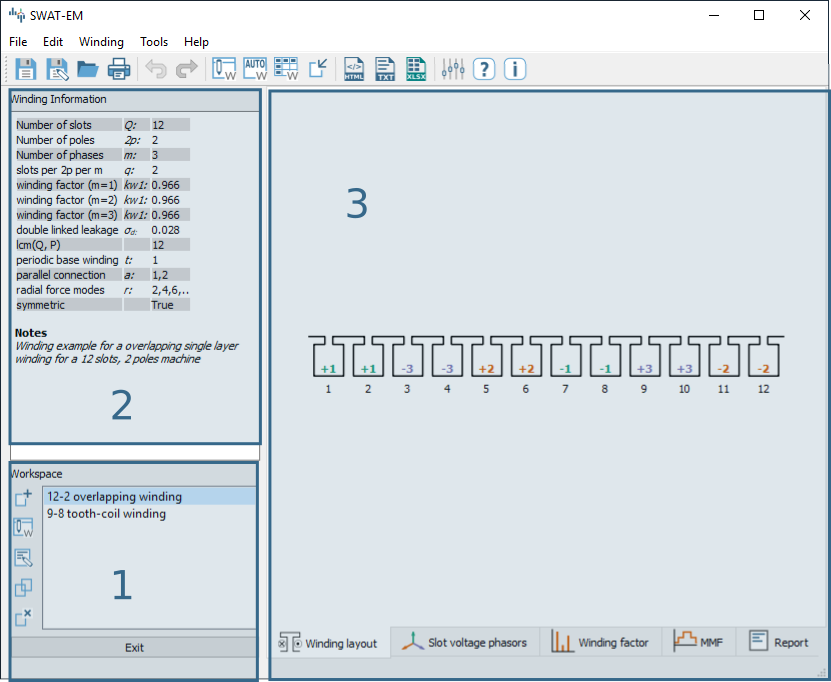
\includegraphics[width=0.99\textwidth,angle=0]{fig/mainwindow}
    \caption{Main-window}
    \label{fig:mainwindow}
\end{figure}
%

\subsection{layout plot}
\subsection{}




\bibliographystyle{unsrt}
\bibliography{literature}

\end{document}







